The weak phase \phis is an important parameter in the \BBbarSyst. It quantifies the third
type of CP-Violation mentioned in \secref{Phenomenology}, nameley in the interference between
two decay amplitudes, see \figref{interference}. In the current section the parameter \phis
and its relevance to the search for new particles is introduced. The status of the \phis
measurements concludes the section.

\newcommand{\ffig}{f}
\newcommand{\phimixfig}{\phi_\text{mix}}
\newcommand{\phifig}{\phi_\text{dec}}
\newcommand{\phibarfig}{\kern 0.15em \overline{\kern -0.15em \phi_\text{dec} \kern -0.60em} \kern 0.60em}
\begin{figure}[h]
  \centering
  \resizebox{0.4\textwidth}{!}{\begin{picture}(0,0)%
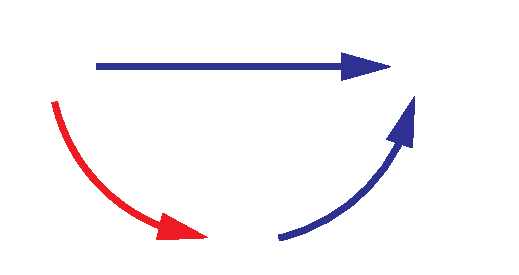
\includegraphics{Figures/Chapter1/decay_CMYK.pdf}%
\end{picture}%
\setlength{\unitlength}{4144sp}%
%
\begingroup\makeatletter\ifx\SetFigFont\undefined%
\gdef\SetFigFont#1#2#3#4#5{%
  \reset@font\fontsize{#1}{#2pt}%
  \fontfamily{#3}\fontseries{#4}\fontshape{#5}%
  \selectfont}%
\fi\endgroup%
\begin{picture}(3939,2094)(2644,-2188)
\put(3286,-736){\makebox(0,0)[rb]{\smash{{\SetFigFont{25}{30.0}{\sfdefault}{\mddefault}{\updefault}{\color[rgb]{0,0,0}$\Bs$}%
}}}}
\put(5761,-736){\makebox(0,0)[lb]{\smash{{\SetFigFont{25}{30.0}{\sfdefault}{\mddefault}{\updefault}{\color[rgb]{0,0,0}$\ffig$}%
}}}}
\put(4501,-421){\makebox(0,0)[b]{\smash{{\SetFigFont{25}{30.0}{\sfdefault}{\mddefault}{\updefault}{\color[rgb]{0,0,1}}%
}}}}
\put(5581,-1771){\makebox(0,0)[lb]{\smash{{\SetFigFont{25}{30.0}{\sfdefault}{\mddefault}{\updefault}{\color[rgb]{0,0,1}}%
}}}}
\put(3331,-1771){\makebox(0,0)[rb]{\smash{{\SetFigFont{25}{30.0}{\sfdefault}{\mddefault}{\updefault}{\color[rgb]{1,0,0}}%
}}}}
\put(4501,-2041){\makebox(0,0)[b]{\smash{{\SetFigFont{25}{30.0}{\sfdefault}{\mddefault}{\updefault}{\color[rgb]{0,0,0}$\Bsb$}%
}}}}
\end{picture}%
}
  \caption{The two interfering decay amplitudes leading to the same final state.
           The phases $\phimixfig$, $\phifig$ correspond to ....
           % This is assuming no CP violation in mixing or CP violation in decay.}
           }
  \label{interference}
\end{figure}

The parameter \phis manifests in the so called $\bquark \rightarrow \cquark\cquarkbar\squark $ transitions, where the
\bquark of the \Bs meson decays into three other quarks, a $\cquark\cquarkbar$ and an $\squark$, see \figref{b2ccs}.
In addtion, the final state of the \Bs meson has to be a CP eigenstate, which implies that both \Bs and \Bsb
can decay into it. The mixing releated phase $\phimixfig$ is governed by the $|\qoverp|$, as shown in \equref{phase_mix}.
Whereas the phase ascociated with the decay comes from the ratio of two decays, shown in \equref{phase_decay}, {\color{red} give ref to both from pdg}, igonoring on shell part of the hamiltonian.

\begin{figure}[h]
  \centering
  {\sffamily \input{Figures/Chapter1/tree}}
  \caption{{\color{red} Fix this to look more like \figref{QuarkMixing} and put ckm elements on the vertices}}
  \label{b2ccs}
\end{figure}

\begin{equation}
 \phimixfig \propto \frac{q}{p} = \sqrt{ \frac{\bra{\Bsb}\ket{\Bs}}{\bra{\Bs}\ket{\Bsb}}} = \frac{\Vtb^*\Vts}{\Vtb\Vts^*}
\label{phase_mix}
\end{equation}

\begin{equation}
 \phifig = \text{arg}\parenthesis{\frac{\bra{f}\ket{\Bs}} {\bra{f}\ket{\Bsb}} } = \text{arg}\parenthesis{\frac{\Vcb\Vcs^*}{\Vcb^*\Vcs}}
\label{phase_decay}
\end{equation}

\noindent A very common parameter that is used to parametrize CP violation in the interference between mixing and decay is shown in \equref{lambda_cpv}.

\begin{equation}
 \lambda_{f} = \frac{q}{p} \frac{\bra{f}\ket{\Bs}} {\bra{f}\ket{\Bsb}} \equiv \frac{||}{}
\label{lambda_cpv}
\end{equation}

Given the so called {\it master equations}{\color{red} ref pdg} for the decay rates of a \Bs and \Bsb
to a final state $f$, the asymmetry due to the interference between mixing and decay\footnote{assuming no CP-Violation
in the \BBbarSyst mixing} is shown in \equref{cpv_interf}

\newcommand{\half}{\frac{1}{2}}
\begin{equation}
  \Acp{\text{inter}} = \frac{ - \Im(\lambda_f) \sin(\Delta m_s t)} {\cosh(\half \Delta\Gamma_s t) - \Re(\lambda_f)\sinh(\half\Delta\Gamma_s t)},
\label{cpv_interf}
\end{equation}


\begin{itemize}
  \item What is it, cartoon diagrams
  \item q over p is equal to
  \item decay part is equal to, feynman diagrams
  \item Assymnetry is equal to
  \item NP in \phis, New particles in the box, new vector boson. Mention some types of models.
\end{itemize}

\subsubsection{Measuring \phis}

\begin{itemize}
  \item Show how do you read phis from the decay time distribution.SHow terms in pdf
  \item \phis status
  \item Higher order effects in view of the current results. Connect with penguin analysis.
\end{itemize}
